\documentclass[journal]{IEEEtran}
\usepackage{graphicx}
\usepackage{booktabs}
\usepackage{cite}
\usepackage{url}
\usepackage{siunitx}
\sisetup{detect-all}

\begin{document}

\title{Parked Loads: Protocol-Safe Wait-Until-Written\\Reads for Multi-Host CXL Memory}

\author{Romyull~Islam
\thanks{Manuscript draft, October 2026. R.~Islam is with Kennesaw State University, Kennesaw, GA,
USA (e-mail: mislam22@students.kennesaw.edu).}}% department to be added

\markboth{IEEE Computer Architecture Letters (draft)}{Islam: Parked Loads for Multi-Host CXL Memory}

\maketitle

\begin{abstract}
Hosts that share a CXL memory device have no cross-host hardware coherence, or only a small
coherent region, so the databases, message passing, GPU collectives and LLM serving systems built on
such memory synchronize by flushing and polling. Every poll is a device access, so waiting threads
consume the bandwidth that other tenants of a memory pool need. Holding a read at memory until the
data is written is an old idea, but a CXL device must do it without breaking the protocol: request
credits are finite, hosts fail independently, and a read that outlives the Root Port's completion
timeout isolates the whole port. We give five rules under which a device parks a CXL.mem read of an
empty line and answers it when another host's write lands, and check them with the TLA+ model
checker: together they rule out Root Port timeouts, stale data and blocked writers, and removing any
one of them breaks one of these guarantees. We implement the device in gem5 and run x86 programs on
up to 36 simulated hosts. Parked waiters issue 1.4 device reads per message instead of 39 to 750,
and with 256 waiters a pooled device keeps over 99\% of its tenants' bandwidth instead of 77 to
79\%.
Handoff latency matches or beats flag polling, and parking a cache-line fill beats the best
software scheme by 1.25$\times$ for one-line messages.
\end{abstract}

\begin{IEEEkeywords}
CXL, memory pooling, synchronization, full/empty bits, multi-host shared memory
\end{IEEEkeywords}

\section{Introduction}
CXL 2.0 switches and multi-headed devices let 2 to 16 hosts load and store the same memory. CXL
3.x adds back-invalidation (BI) for hardware coherence, but deployments keep the coherent region
small or absent, and shared memory exposed as HDM-H supports only software coherence~\cite{cxl3}.
Cross-host communication therefore runs on software protocols: a producer writes a message and a
flag, the consumer flushes its cached copy and re-reads the flag until it changes. Every system
built on shared CXL memory so far waits this way. A distributed database for a CXL pod keeps its
locks in the small coherent region~\cite{tigon}; MPI and RPC over CXL poll message
queues~\cite{cmpi,hydrarpc}; GPU collectives spin on a doorbell per chunk~\cite{cccl}; and TraCT,
which hands KV cache from prefill to decode servers through CXL memory for LLM serving, polls and
flushes lock state per node: acquiring a lock takes 20 to 100\,\si{\micro\second} from 2 to 16
nodes in its simple design and below 40\,\si{\micro\second} in its optimized
one~\cite{tract,tract_thesis}. Software coherence also
limits which synchronization schemes can be expressed at all~\cite{pnnlsync}. Measured costs
are high. On an FPGA multi-headed device a flushed access takes \SI{2.2}{\micro\second}, 2.8$\times$
a cached one, and \texttt{clflush} plus fence costs 2 to \SI{3}{\micro\second}~\cite{cmpi}; a
64\,B RPC round trip takes \SI{1.47}{\micro\second} on a \SI{300}{\nano\second} device~\cite{hydrarpc};
a switch adds at least \SI{220}{\nano\second} per access~\cite{octopus}; a characterization of
multi-host CXL 2.0 on commercial hardware finds up to 4$\times$ the latency of local DRAM and
cross-host write visibility that depends on carefully chosen flush and fence patterns~\cite{damon26}; and loaded latency rises
from 230 to \SI{1624}{\nano\second} under contention~\cite{memchannel}.

Polling has two costs. The waiter learns of the write only on its next poll, after a device round
trip and, with a flush, later still. And each poll is a device access, so waiting threads consume
bandwidth that other tenants of a shared pool need. The device is the only place that sees both the
waiting read and the releasing write, so it can answer the read when the write lands. Holding a
read in memory until it can be satisfied is not new: HEP and the Tera MTA~\cite{tera} and
I-structures~\cite{istructures} queued reads of empty locations, and IBM's conditional load with
timeout holds a load in a memory controller until a store arrives or a timer
expires~\cite{ibmclt}. We do not claim the waiting primitive. We claim that it can be made safe on
CXL.mem, which no prior design faces: the waiter and the writer are independent hosts behind a
switch or a multi-headed device, request credits are finite, a read must not outlive a completion
timeout whose expiry isolates the port, the protocol has no response that means \emph{not yet}, and
hosts fail separately.

This letter contributes (1) five rules under which a CXL device parks a CXL.mem read without
breaking forward progress, ordering or timeouts, and the host rules that make parking work with
caches and prefetchers; (2) a TLA+ model~\cite{tla} that the TLC model checker~\cite{tlc} uses to
show the rules sufficient and each one necessary; and (3) an implementation of the device in
gem5~\cite{gem5}, with x86 programs on up to 36 hosts, measuring latency and the fabric bandwidth
that polling waiters take from other tenants of a shared device.

\section{Parked loads}
\textbf{Synchronization region.} The fabric manager marks an HDM range as a synchronization region.
The device keeps one full/empty bit per 64\,B line, in SRAM for small regions (\SI{128}{\kilo\byte}
covers \SI{64}{\mega\byte}) or in spare metadata bits. A write to a line stores the data, sets it
\emph{full} and answers the reads parked on it. The region is reachable through a second address
window in which a read is \emph{consuming} (it also sets the line empty, for single-consumer queues)
and a write sets the line empty.

\textbf{Rule 1: parking frees the request credit.} A read of an empty line moves from the request
queue into a parked table keyed by line address. CXL returns a request credit when the receiver
frees the buffer holding the message~\cite{cxl3}, so other requests keep flowing. Responses need no
device credit: NDR and DRS buffers are preallocated at the requester~\cite{cxl3}.

\textbf{Rule 2: the releasing write is never blocked.} Writes travel on the RwD channel, which must
pass the request channel~\cite{cxl3}. CXL places no ordering between message classes or between
addresses, so answering a parked read after later requests is legal; a device already holds reads
to lines with an outstanding back-invalidate snoop~\cite{cxl3}.

\textbf{Rule 3: every parked read is answered before the Root Port times out.} A read parked past
the completion timeout makes the Root Port synthesize a poisoned response and isolate the
port~\cite{cxl3}. The timeout is programmable from \SI{50}{\micro\second}, so the device answers
every parked read within $\tau=\SI{25}{\micro\second}$.

\textbf{Rule 4: the answer says \emph{not yet}.} CXL has no such response: DRS carries only MemData
and MemData-NXM. The device returns the line's current contents, and software sees an unchanged
sequence number and re-issues, so a long wait costs one access per $\tau$ instead of one per round
trip; a reserved metadata value (HDM-H metadata is host defined) or a new DRS opcode can mark it
explicitly. A full table answers at once, which degrades to polling.

\textbf{Rule 5: a read for ownership is never parked.} A store that misses in a write-back mapping
first reads the line for ownership; parking that read would block the writer until $\tau$. An HDM-H
device cannot tell such a read from a shared one unless the host marks it in the metadata bits, so
writers update sync lines with non-allocating stores (uncached, or a full-line
MOVDIR64B~\cite{intelsdm}), and the device answers marked ownership reads at once.

\textbf{Host side.} A waiter can park in two ways. An \emph{uncached} load of a flag never issues
speculatively. A \emph{cacheable} line fill parks as well: the waiter flushes its copy and loads the
line, and the wake-up delivers the whole 64\,B line, so a message of one line arrives with the
wake-up. A speculative or prefetched fill only holds a miss buffer until the wake-up or $\tau$, but
two host rules keep it harmless: cacheable parked reads are non-consuming (a prefetch must not take
a message; the waiter empties the line afterwards with a store to the consuming window, off the
critical path), and each sync line sits on its own 4\,KiB page, which hardware prefetchers do not
cross, so a writer's store never merges behind its own parked prefetch. A parked load stalls only
its thread, which would otherwise spin.

\textbf{Failures, fairness and cost.} When a host fails or its logical device is reset, the device
drops that host's entries; waiters of a failed producer see \emph{not yet} every $\tau$ and apply
their lease logic. Wake-up is FIFO per line. An entry holds the line address, the requester's port
and tag and a timer, under 16\,B; 4,096 entries take \SI{64}{\kilo\byte}.

\textbf{Prior art.} Memory-side waiting is old. IBM's conditional load with timeout keeps pending
loads in a memory-controller table with a timer and replies when a store satisfies the condition or
the timer (0.5\,\si{\micro\second} in its example) expires~\cite{ibmclt}; Microsoft's conditional
synchronization adds a similar memory-side timeout~\cite{msftcond}; the Synchronization State
Buffer keeps full/empty state only for locations being synchronized~\cite{ssb}; QOLB queues waiters
in hardware~\cite{qolb}; Lustig and Martonosi hold GPU reads until a CPU write and name timeouts as
future work~\cite{lustig}; Callback blocks on-chip reads in a directory~\cite{callback}. All of them
live inside one machine, where the waiter and the writer share a memory controller and no fabric
timeout or credit rule applies. In CXL, Intel's patents queue contended atomics and keyed lock
requests in a device~\cite{intelq,intellock} or forward MONITOR/MWAIT to a remote home
node~\cite{intelmwait}, and Micron's device defers requests to busy cache lines~\cite{micron}; none
holds a plain read until another host writes the data, and none derives the bound from the Root
Port timeout.

\section{Verification}
The TLA+ model has consumer hosts that wait on a sync line, a producer that first reads an ordinary
line and then writes the sync line (possibly through a write-back mapping, so with a read for
ownership), request credits, the RwD channel, a bounded parked table, the device timeout and the
Root Port timeout. The producer may wait arbitrarily long and may fail; time advances only when no
other step is possible, and credit arbitration is fair. TLC checks four invariants (no read
outlives the Root Port timeout; a consumer never accepts unwritten data; the producer's ordinary
read and its releasing write never wait as long as $\tau$) and one liveness property (if the
producer lives, every consumer gets the data), for 2 and 3 consumers sharing 2 credits and a
2-entry table. With all five rules every property holds (up to 8,572 states). Removing a rule
breaks exactly what it protects (Table~\ref{tab:tlc}). Rule 2 alone is redundant once Rule 1 holds,
because a parked read then holds no credit; CXL provides it anyway.

\begin{table}[t]
\centering
\caption{Model-checking results (2 and 3 consumers): the property TLC finds violated when a rule
is removed.}
\label{tab:tlc}
\footnotesize\setlength{\tabcolsep}{3pt}
\begin{tabular}{ll}
\toprule
Rules & Violated property (shortest trace) \\
\midrule
all five & none; liveness holds \\
without R1 & producer's ordinary read waits $\tau$ (8 states) \\
without R1, R2 & releasing write also waits $\tau$ (11 states) \\
without R2 & none (R1 implies it) \\
without R3 & read outlives the Root Port timeout (9 states) \\
without R4 & consumer accepts stale data (8 states) \\
without R5 & write-back writer waits $\tau$ (17 states) \\
\bottomrule
\end{tabular}
\end{table}

\section{Evaluation}
\textbf{Setup.} We add the device to gem5 v25.1~\cite{gem5} as a memory object: SimpleMemory timing
(\SI{100}{\nano\second} access, \SI{64}{\giga\byte\per\second} port, at least one 64\,B line per
access), full/empty bits, two address windows, a parked table and the timeout. Each host is its
own gem5 system with out-of-order x86 cores (in-order for barriers and waiters), 32\,KiB L1s, a
1\,MiB L2 with a stride prefetcher and its own coherence domain; hosts reach the device through a
link with a flight delay and \SI{32}{\giga\byte\per\second}, meeting at a shared crossbar. The idle
round trip is \SI{124.5}{\nano\second} plus twice the flight delay, which we set to model a
\SI{250}{\nano\second} expander, a \SI{280}{\nano\second} multi-headed device and a
\SI{600}{\nano\second} switch~\cite{octopus,cccl}. Static x86 programs run on every host and time
handoffs with the simulated clock. Protocols: \emph{flush} poll (clflushopt, fence, load of a
flag), \emph{uncached} poll, \emph{line} poll (re-read the payload lines until all carry the new
sequence number, the fastest software scheme), \emph{parked flag} (uncached) and \emph{parked line
fill}. gem5 charges a flush only its cache work, while hardware pays up to
\SI{1.4}{\micro\second}~\cite{cmpi}, so polling here is the cheap case. As a cross-check, our earlier
discrete-event model gives 890\,ns for flag polling of a 64\,B message on the expander and gem5
944\,ns.

\begin{figure}[t]
\centering
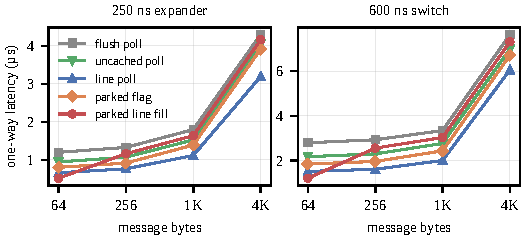
\includegraphics[width=\columnwidth]{fig_latency.pdf}
\caption{One-way handoff latency in gem5, consumer already waiting.}
\label{fig:lat}
\end{figure}

\textbf{Latency.} For one-line messages a parked line fill is fastest on every device
(Fig.~\ref{fig:lat}): 517, 577 and 1,216\,ns, 1.25 to 1.27$\times$ faster than line polling,
1.8$\times$ than uncached and 2.3$\times$ than flush polling. Longer messages need a doorbell and a
payload read, and a write-back store first reads the line for ownership, so line polling is fastest
there; the parked flag is still 1.04 to 1.17$\times$ faster than uncached and 1.1 to 1.5$\times$
faster than flush polling, and so it is for RPCs (3.9 versus 4.6 and 5.7\,\si{\micro\second} for a zero-work
call on the switch). Barrier rounds are unchanged (3.7\,\si{\micro\second} for 4 hosts on the
switch with a parked or uncached flag), because the master's sequential scan of arrival flags, one
round trip each, dominates. Full-line non-temporal stores, which gem5 does not model, would remove
the ownership read.

\begin{figure}[t]
\centering
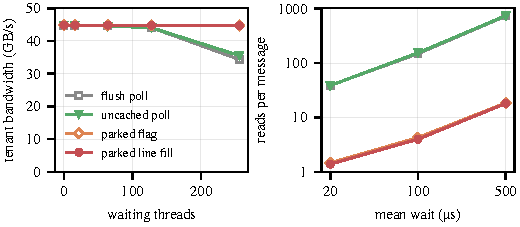
\includegraphics[width=\columnwidth]{fig_contention.pdf}
\caption{Left: bandwidth of four streaming tenant hosts on the switched device next to waiting
threads (messages every \SI{20}{\micro\second} on average). Right: device reads per message for 64
waiters as the mean wait grows past $\tau$.}
\label{fig:cont}
\end{figure}

\textbf{Shared-device contention.} Four tenant hosts stream reads at 44.9\,GB/s alone. Next to 256
polling waiters they drop to 34.3 (flush) and 35.5\,GB/s (uncached), because every waiter issues a
device read per round trip, 39 per message (Fig.~\ref{fig:cont}). Parked waiters issue 1.4 to 1.5
reads per message, the tenants keep 44.6 to 44.8\,GB/s, and handoff stays at 1.25 (line fill) and
1.93\,\si{\micro\second} (flag) against 2.25 and 2.88\,\si{\micro\second} for polling. When the mean
wait grows to \SI{500}{\micro\second}, far beyond $\tau$, a parked read times out and re-parks every
\SI{25}{\micro\second}: 18 reads per message against 740 to 750 for polling, at unchanged handoff
latency. A table smaller than the number of waiters degrades toward polling: with 128 or 32 entries
for 256 waiters, overflowing reads are answered at once and retried (13 to 32 reads per message),
and the tenants keep 43.8 to 44.0 and 38.0 to 39.1\,GB/s, still more than with polling.

\textbf{Limitations.} gem5 runs the programs in syscall-emulation mode, models the switch as a
crossbar and does not model back-invalidate coherence or full-line non-temporal stores; hardware
flushes cost more than gem5 charges, which favors polling. The TLA+ model is checked for small
configurations.

\section{Conclusion}
A CXL memory device is the one point that sees a waiting read and the write that satisfies it.
Memory-side waiting is old; this letter shows that a multi-host CXL device can do it within
CXL.mem's credit, ordering and timeout rules, proves with a model checker that five rules suffice
and each is needed, and shows in gem5 that parked waiters stop consuming a pooled device's
bandwidth (1.4 instead of 39 to 750 reads per message) while matching or beating polling latency.

\bibliographystyle{IEEEtran}
\bibliography{p3}

\end{document}
